\documentclass[../main.tex]{subfiles}
\begin{document}
\subsection{Comparing different radii}
The first objective we set was determining the optimal beacon range.
For this we tested all datasets, ceteris paribus, with the following levels of beacon radius: 0.25 till 3 with increments of 0.25 and also a radius of 0.1.  
In figure \ref{fig:rad} we see the results of this tests where we took averages across all datasets.
The figure clearly indicates a minimum at a beacon radius of 0.75.
\begin{figure}
	\centering
	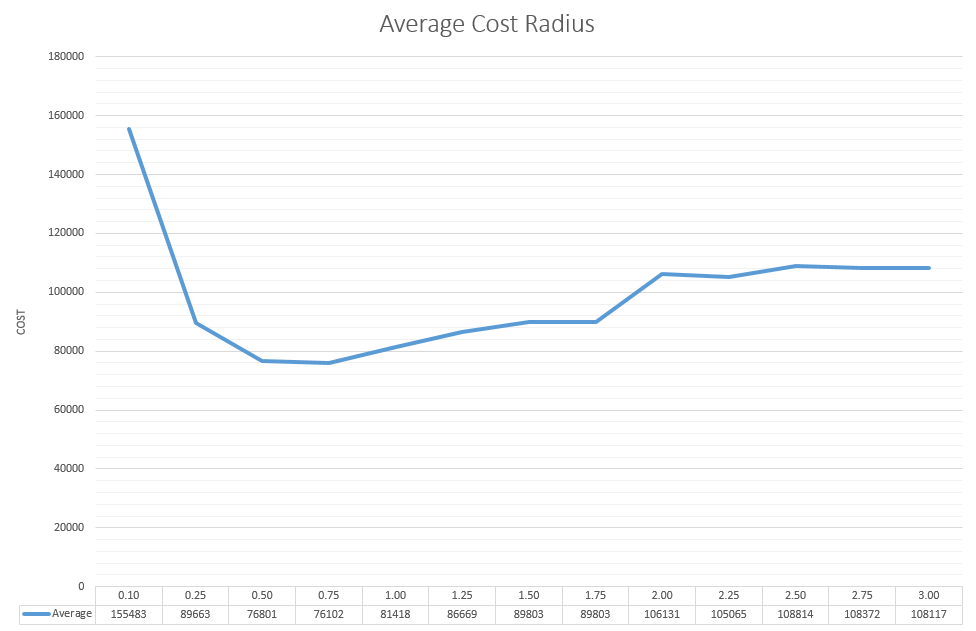
\includegraphics[width=\textwidth]{radiusaveragecost.png}
	\caption{The averages taken over all dataset per beacon radius with the given levels.}
	\label{fig:rad}
\end{figure}

\subsection{Comparing exchange versus no exchange}
One of the objectives is to find out whether exchanging parcels between agents is benifical with respect to the objective function.
In figure \ref{fig:exch} the results of running all data sets, ceteris paribus, with and without exchanges enabled are displayed.
There is no clear difference which choice is better only 8 of the 15 datasets yields better results with the exchanges enabled.
Neither the averages in table \ref{tab:avgstrat} show a clear difference between the two cases.
Note however that this could be due to the way we implemented the exchange. 
The implemenation is quite naive and tries to exchange very often. 
An improvement could be looking at how much distance would be covered between the parcels in both agents and only exchange if the new clustering would improve this number.
Of course this would have to take the distance to drive for the exchange into account.
This could then probably eliminate a whole lot of unnecessary exchanges and reduces the cost.

\begin{figure}
	\centering
	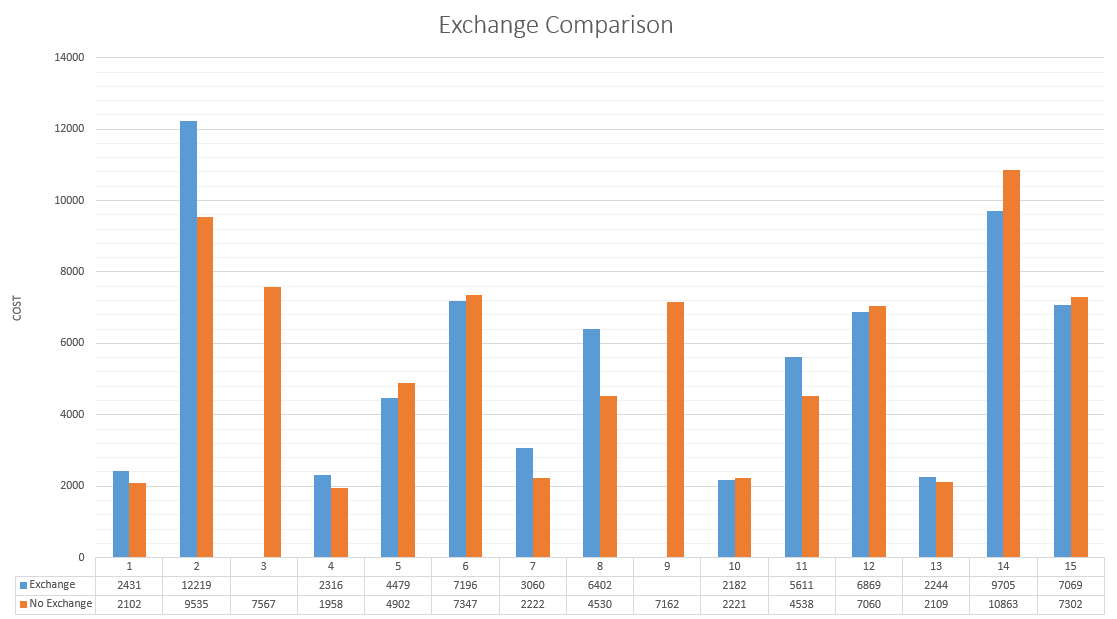
\includegraphics[width=\textwidth]{exchangecomp.png}
	\caption{Visual representation of comparing experiments with and without exchanges between agents.}
	\label{fig:exch}
\end{figure}


\subsection{Comparing exchange strategies}
The third and last objectivce was determining how a delivery strategy improves the solution.
In figures \ref{fig:stat_ex} and \ref{fig:strat_noex} we can clearly see that NearestOnTimeDeliveryStrategy is, outliers excluded, consitently better. 
This is also very easy to see in table \ref{tab:avgstrat} where we find in both the exchange and no exchange case it is clearly the lowest average.
Second in place would be the NearestDeliveryStrategy although the difference with the last place is not as clear compared to the first place.
\begin{figure}
	\centering
	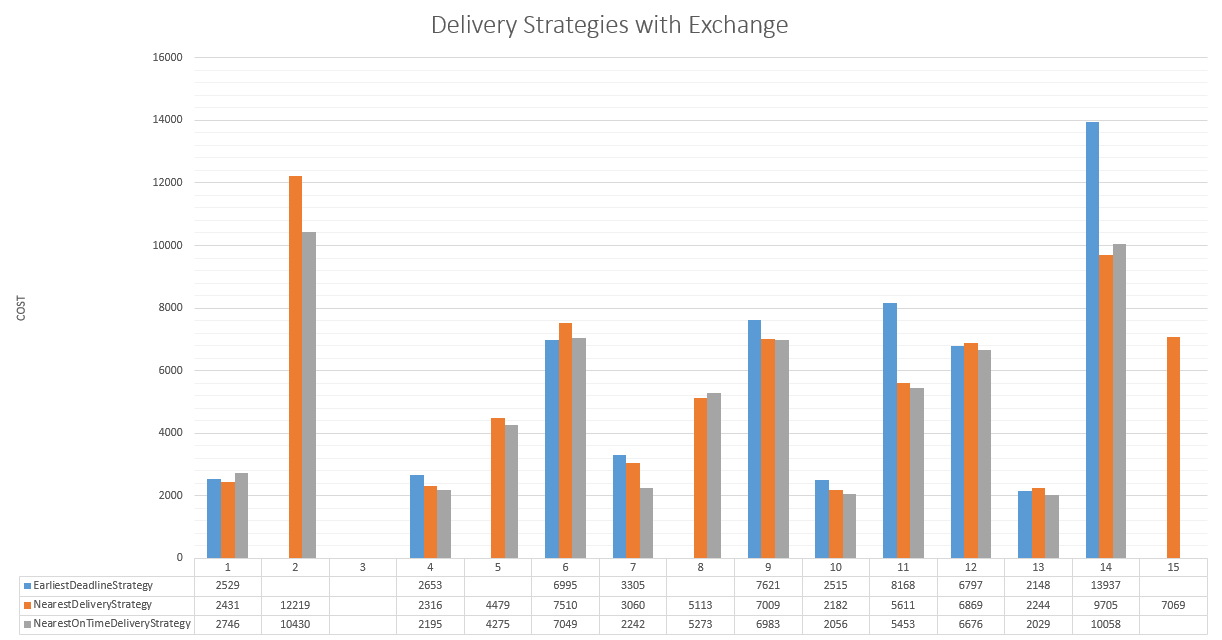
\includegraphics[width=\textwidth]{exchangestrategy.png}
	\caption{The averages taken over all dataset per beacon radius with the following levels:}
	\label{fig:strat_ex}
\end{figure}

\begin{figure}
	\centering
	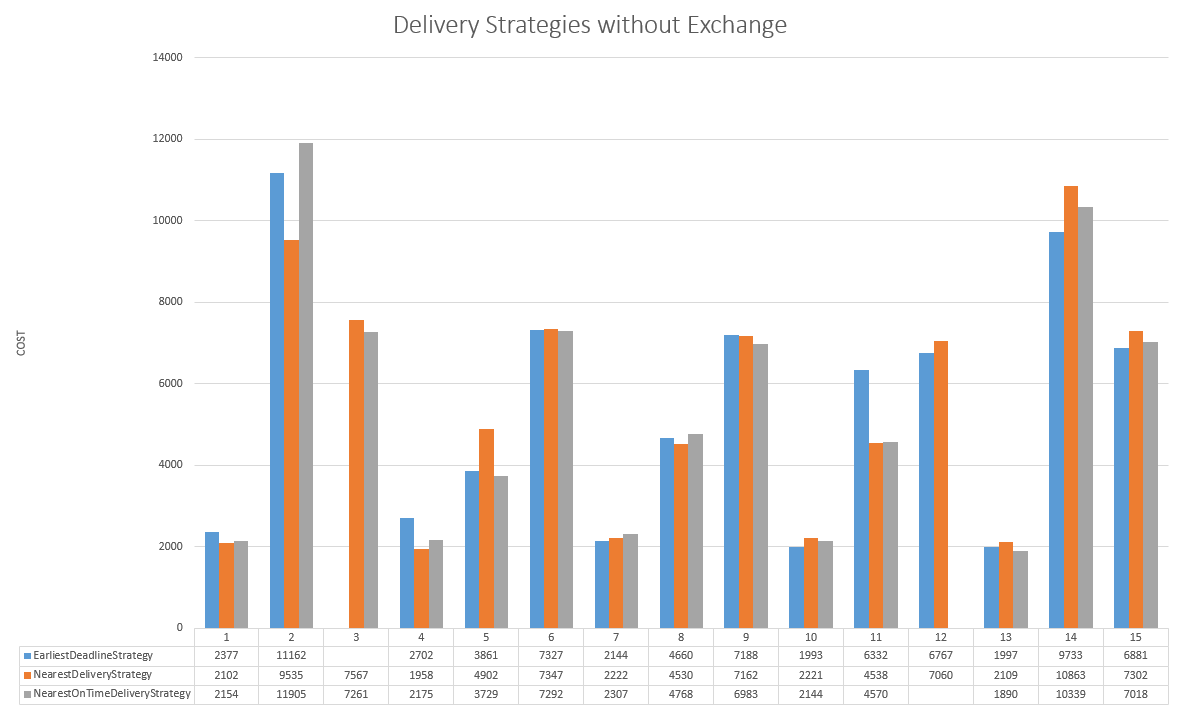
\includegraphics[width=\textwidth]{noexchangestrategy.png}
	\caption{The averages taken over all dataset per beacon radius with the following levels:}
	\label{fig:strat_noex}
\end{figure}
\begin{table}
\begin{tabular}{lcc}
	\toprule
	& Without Exchange & With Exchange \\ 
	\midrule
	EarliestDeadlineStrategy & 5366 & 5666.8 \\ 
	NearestDeliveryStrategy & 5427.867 & 5558,357 \\ 
	NearestOnTimeDeliveryStrategy & 5323.929 & 5189.615 \\ 
	\bottomrule
\end{tabular}
\caption{Table with averages of the different delivery strategies across the all data sets.}
\label{tab:avgstrat}
\end{table}

\end{document}
